\chapter{Clustering} \label{chap:chap-2}

% if you want a short header you can use the following command
% \chapter[short-header-name]{chapter-title} \label{chap:chap-2}


% if you want to add the quote above the chapter heading then do the following:
% (for this case, you may have to change \ChapterTopSpace in the main file)
% \epigraphhead[0]{whole-above-epigraph-goes-here}


% add the citation for the chapter if it is a reprint


% add your chapter text here
\section{Introduction}
Given the capabilities and limitations of SDLs, quick and accurate characterization of the electrical compounds produced is needed. Clustering experimental results becomes crucial for several reasons. 
Clustering identifies patterns and similarities among experimental results. This aids in the discovery of underlying trends or relationships between different compounds or experimental conditions. It also facilitates quality control by pinpointing outliers or anomalies in experimental data, ensuring the reliability of SDL data. 

Moreover, clustering allows researchers to optimize processes by providing insights into the effects of various parameters, such as metal/ligand ratio, on the formation of redox or electrochemical compounds. This optimization can significantly enhance the efficiency of voltammetry automation in SDLs. Additionally, by classifying different types of electrical compounds based on their properties or characteristics, clustering supports classification and prediction tasks, enabling researchers and SDLs to predict the behaviour of new compounds or classify unknown compounds based on their similarities to known clusters. Categorizing the automated characterizations typically done by SDLs can improve the automation capabilities of the laboratory. This is done by improving the behaviour mapping of a certain compound under certain conditions into a chemical space. 
Finally, clustering provides a structured way to organize and interpret large volumes of experimental data, facilitating decision-making processes related to the selection of compounds for further analysis or the design of future experiments. In essence, clustering experimental results in the context of SDLs used for voltammetry is indispensable for gaining insights, ensuring data quality, optimizing processes, classifying compounds, and facilitating decision-making processes, which are crucial in an SDL environment.
\section{Data Collection}
To analyze how data gathered from SDLs can be clustered, this work uses an open dataset published by the Aspuru-Guzik group \cite{PabloGarca2024}. The data was collected through autonomous electrochemistry experimentation that operates through an iterative workflow \cite{PabloGarca2024}. The workflow was used to synthesize ten distinct metals and ten distinct ligands, with specific details available in Appendix \ref{metal_table} and Appendix \ref{ligand_table}, resulting in 100 unique complexes. Each complex was synthesized using a metal/ligand concentration ratio of 1:7 to ensure complete complexation. The synthesis process employed 1.0 M NaCl in water as the electrolyte/solvent and a buffer solution consisting of a 1:1 ratio of HOAc/NaOAc. Following synthesis, comprehensive characterizations were conducted using CV and DPV techniques. The experimentation was done using a low-cost electrochemistry platform designed as an alternative to commercial options. The number of points in each sample can vary due to different scan rates or voltage windows. Higher scan rates lead to more data points being collected during the experiment and can provide finer resolution of the electrochemical processes occurring. Additionally, it\textquotesingle s worth noting that these samples may be duplicated as CV and DPV analyses can be conducted multiple times on the same sample to ensure robustness. Notably, the workflow is adaptable, with the potential to encompass a broader range of parameters, including additional ligands, varying metal/ligand ratios, and reaction times. Mixed ligands and different buffer pH levels can also be configured but was not done so for this dataset. The accumulation of data points is ongoing, contributing to the continuous expansion and refinement of our understanding. The final dataset consists of 800 CV and 200 DPV data points. The dataset used in this work can be found on \href{https://zenodo.org/doi/10.5281/zenodo.10633135}{Zenodo}.
\section{Curse of Dimensionality}
The curse of dimensionality refers to the phenomena that cause various challenges and complications when analyzing data in high-dimensional spaces. As the number of features in a dataset expands, the volume of data required to generalize accurately grows exponentially \cite{Bellman2003-by}. With each additional dimension, the data becomes sparser, posing significant hurdles for tasks like clustering and classification. In higher dimensions, the distinction between distances among data points diminishes, making measurements like Euclidean distance negligible. As such, algorithms that rely on distance measurements will experience a drop in performance. Furthermore, more dimensions will require more computational resources and time to process the data. It is good practice to aim to have the data in as low a dimension as possible, provided that relevant information is maintained. 
\section{Ramer–Douglas–Peucker Algorithm}
\begin{figure}[!h]
  \centering
    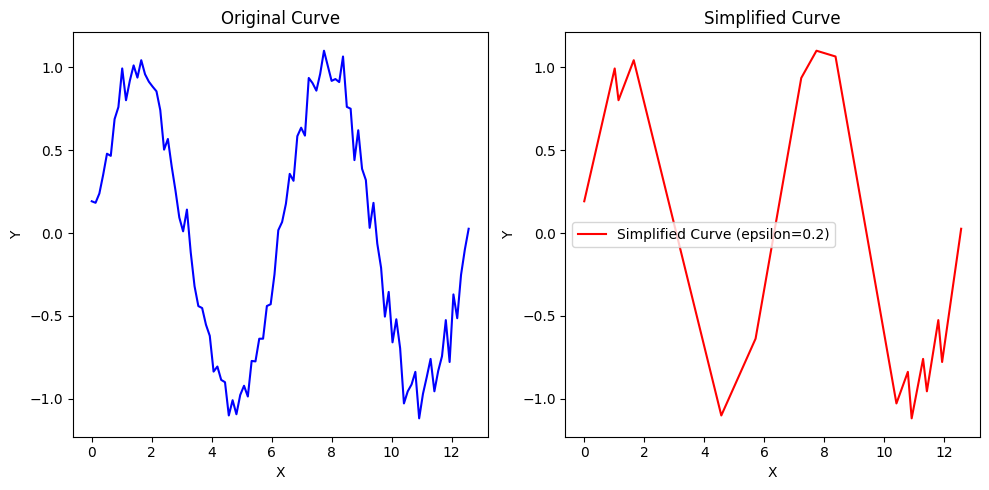
\includegraphics[width=1.0\textwidth]{figures/rdp.png}
    \caption{RDP Algorithm}
    \label{rdp}
\end{figure}
The Ramer–Douglas–Peucker (RDP) algorithm is employed to reduce the number of points in a curve approximated by a series of points \cite{Wu2004-gc}. It operates by conceptualizing a line between the initial and terminal points within the curve\textquotesingle s points. Subsequently, it identifies the point furthest from this line among the intermediary points. If this point, termed the outlier point, and consequently all intervening points, lie within a specified distance $\epsilon$ from the line, they are removed. Conversely, suppose the outlier point exceeds the $\epsilon$ distance. In that case, the curve is segmented into two parts: from the initial point to the outlier point, inclusive and the outlier and the remaining points. The algorithm is then recursively applied to both resulting segments, and the reduced forms of the curve are reassembled. Figure \ref{rdp} shows curve simplification done with the RDP algorithm. Since CV and DPV results can be represented as a curve, RDP can be used to remove unnecessary points while maintaining the overall shape of the voltammogram. This will reduce the dimensionality and improve data analysis results.
\section{Data Preparation and Encoding}
Many parameters can be set during CV and DPV analysis, affecting the characterization outcomes. Notably, the experiment\textquotesingle s scan rate affects the sampling frequency and the number of points collected within a specific time interval, leading to a variable number of point densities depending on the analyzed compound. Heterogeneity among samples becomes challenging for many ML algorithms, as they often require input data to be the same shape. Similarly, the potential limit at which the potential begins to return to its initial point will affect the overall shape of the cyclic voltammogram. To address these issues, the following steps are used to encode the data:
\begin{enumerate}
    \item Split experiment cycles into separate data points.
    \item Normalize values to fit between [0, 1].
    \item Reduce points using the Ramer-Douglas-Peucker algorithm.
    \item Duplicate data points until the total length reaches the longest cycle\textquotesingle s length.
    \item Order data points based on angular position relative to the center.
\end{enumerate}
Due to the curse of dimensionality, the RDP algorithm is used to reduce the number of dimensions. Since the RDP algorithm takes only a variable $\epsilon$, the final length after reduction will differ for each data set. Data points are randomly selected and duplicated to ensure the data is the same size as the longest after RDP reduction. Finally, the data is ordered based on its angular position relative to the center for consistency.
\begin{figure}[!h]
  \centering
    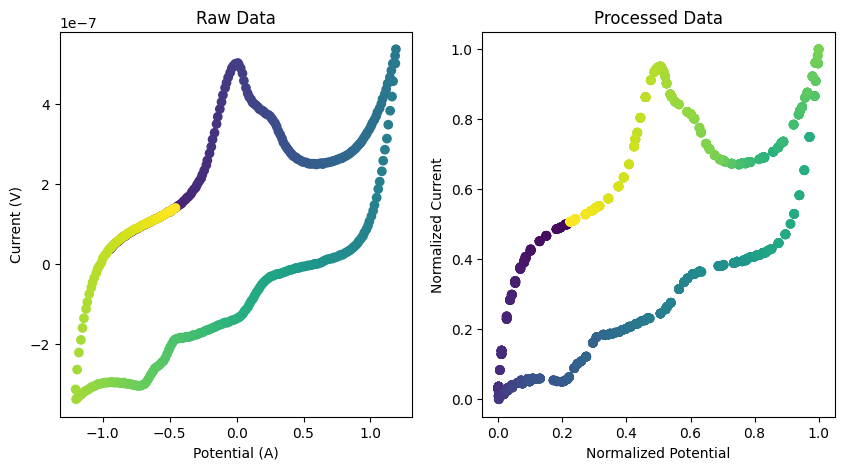
\includegraphics[width=1.0\textwidth]{figures/encoding.png}
    \caption{Raw Data and Processed Data}
    \label{encoding}
\end{figure}
Plots of the raw and processed data can be seen in Figure \ref{encoding}, with the colour of the scatter plot representing time sequence of the points. The starting point and end point varies across different voltammetry experiments. As such, it is important to order the data points so that comparisons can be informative. A significant reduction in dimensionality by 1/3 can also be seen in the plots. Despite this, the important characteristics of the voltammogram, such as the overall shape and peaks, are maintained.
\section{K-Means}
\begin{figure}[!h]
  \centering
    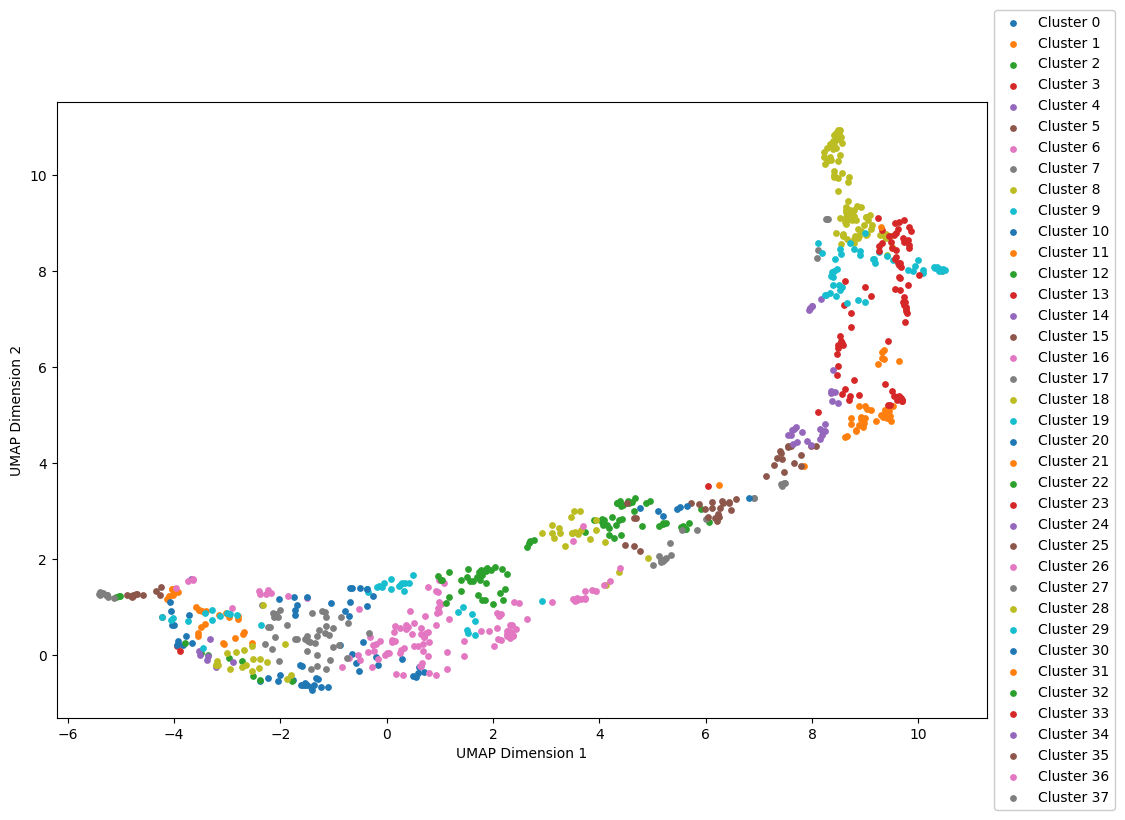
\includegraphics[width=1.0\textwidth]{figures/k-means.png}
    \caption{K-Means Clustering Visualization with CV data}
    \label{kmeans}
    Due to the dimensionality of the data, UMAP (see subsection \ref{chap-2:umap}) was applied to reduce the dimensions of the data.
\end{figure}
K-Means clustering is an unsupervised machine learning algorithm aimed to divide data points into clusters so that the data points within each cluster are similar and different from the data points in other clusters \cite{MacQueen1967}. The K-Means clustering result for CV data can be seen in Figure \ref{kmeans}. The algorithm is explained below, with K representing the desired number of clusters:
\begin{enumerate}
    \item Initially, K points are selected randomly as the cluster centroids.
    \item Each data point is assigned to the closest mean, quantified by the Euclidean distance. 
    \item Each cluster centroid is updated to reflect the average of data points currently assigned to that cluster.
    \item This process is repeated for a specified number of iterations.
\end{enumerate}
One of the questions that needs to be answered is the choice of K. This means finding a balance between the number of clusters represented by K and the average variance of the clusters while minimizing both. There is no approach for determining K that works better than all others. For this problem of clustering CV and DPV data, a combination of the Elbow Method \cite{Thorndike1953} and Silhouette method is used \cite{ROUSSEEUW198753}. The Elbow Method is performed by plotting the within-cluster sum of squares (WCSS) for a range of K and choosing the value K where adding more clusters does not significantly decrease the WCSS. While the Elbow Method can quickly eliminate many values of K, it also has drawbacks regarding the shape of the WSCC curve. Determining the exact location of the \enquote{elbow} can be subjective and depends on the analyst\textquotesingle s interpretation. Different individuals may identify different elbows, leading to inconsistency in results. In cases where the relationship between the number of clusters and WCSS is not distinctly elbow-shaped, the Elbow Method may not provide clear guidance for choosing the appropriate number of clusters.

The Silhouette Method addresses some of these drawbacks by providing a more quantitative measure of cluster quality. Instead of relying on subjective interpretation, the Silhouette Method calculates the silhouette coefficient for each data point, quantifying how similar an object is to its cluster compared to others. This provides a more objective measure of cluster cohesion and separation. The process for selecting K for this work includes determining a set of candidate K values using the Elbow Method by eliminating suboptimal values and then using the Silhouette method to find optimal K among the potential candidates. 
\section{Density-Based Spatial Clustering of Applications with Noise}
\begin{figure}[!h]
  \centering
    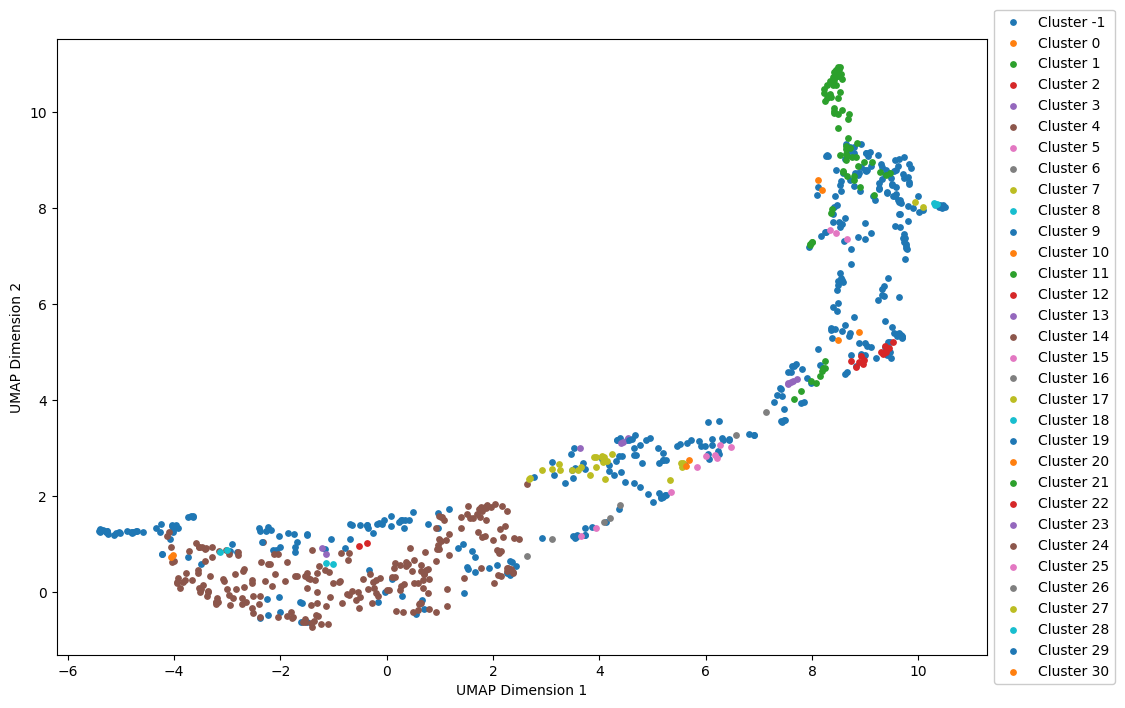
\includegraphics[width=1.0\textwidth]{figures/dbscan.png}
    \caption{DBSCAN Clustering Visualization with CV Data}
    \label{dbscan}
    UMAP (see subsection \ref{chap-2:umap}) was applied to reduce the dimensions of the data.
\end{figure}
Density-Based Spatial Clustering of Applications with Noise (DBSCAN) is another clustering algorithm that works by partitioning the data into dense regions of points separated by less dense areas \cite{Ester1996ADA}. It defines clusters as areas of the dataset with many points close to each other, while the points far from any cluster are considered outliers or noise. In DBSCAN, $\epsilon$ represents the maximum distance between two points for them to be considered neighbours, and minimum samples represents the number of points required for a point to be considered a core point. Points that have fewer than minimum samples points are labelled as noise. The key differentiator for DBSCAN is that the number of clusters does not need to be determined beforehand.  
\section{t-Distributed Stochastic Neighbour Embedding}
Dimensionality techniques like t-Distributed Stochastic Neighbour Embedding (t-SNE) are used for visualizing high-dimensional data in a low-dimensional space \cite{vanDerMaaten2008}. This visualization can aid in the clustering process by providing insights into the underlying structure of the data and help in understanding the results of the clustering algorithm. The first step of the algorithm is to create a probability distribution that represents the similarity between neighbours. The similarity between the two data points is represented by their Euclidean distance. Each data point is placed in the middle of the Gaussian curve, and the rest of the data is placed along the curve. This is represented by the following equation where $j \neq i$ and $p_{i|i} = 1$:
\begin{align}
p_{j|i} = \frac{exp(-||x_i - x_j||^2 / 2\sigma_i^2)}{\sum_{k \neq i}exp(-||x_i - x_k||^2 / 2\sigma_i^2)}
\end{align}
"The similarity of datapoint $x_j$ to datapoint $x_i$ is the conditional probability, $p_{j|i}$, that $x_i$ would pick $x_j$ if neighbours were picked in proportion to their probability density under a Gaussian centred at $x_i$" \cite{vanDerMaaten2008}. The remaining variable, sigma, is not chosen directly but rather by selecting a value for perplexity. Perplexity is defined as:
\begin{align}
Perp(p) \coloneq 2^{-\sum_x p(x)log_2(p(x))}
\end{align}
Perplexity represents the density of data and how many neighbours the central point should have with higher values relating to higher variance. After choosing the perplexity value, the corresponding sigma values are found using binary search. 
Next, the similarities between data points for low-dimensional representations must also be found to ensure that similar data are close after projection. 
\section{Uniform Manifold Approximation and Projection} \label{chap-2:umap}
Uniform Manifold Approximation and Projection (UMAP) is a dimension reduction technique that can be used for visualization similarly to t-SNE \cite{https://doi.org/10.48550/arxiv.1802.03426}. It achieves this by leveraging concepts from algebraic topology and Riemannian geometry.
Here\textquotesingle s a simplified breakdown of how UMAP works:
\begin{enumerate}
\item Constructing a Topological Representation: UMAP starts by creating a fuzzy topological representation of the data. This involves building a simplicial complex, which is a way to represent topological spaces using simple geometric shapes called simplices. The algorithm constructs these simplices based on the proximity of data points.
\item Optimizing Low-Dimensional Representation: Once the topological representation is established, UMAP optimizes a low-dimensional representation of the data to match this topological structure as closely as possible. It does this by minimizing a measure called cross-entropy, which quantifies the difference between the fuzzy topological structures of the high-dimensional and low-dimensional data.
\item Efficient Computations: UMAP employs several strategies to make computations efficient. It focuses on computing only the nearest neighbours of each point and uses algorithms like Nearest-Neighbour-Descent for this purpose. Additionally, it utilizes stochastic gradient descent for optimization and smooth approximations of the membership strength function to ensure differentiability.
\item Preserving Topological Structure: The goal of UMAP is to ensure that the low-dimensional representation maintains the essential topological properties of the original data. It achieves this by balancing attractive forces that pull similar points together and repulsive forces that push dissimilar points apart based on the weights of edges in the topological representation. The farther away the two points are, the more dissimilar they are. 
\end{enumerate}
Overall, UMAP\textquotesingle combination of computational efficiency, scalability, flexibility in parameter tuning, and interpretability make it an appealing option over t-SNE. 
\section{Results and Discussion}
The K-Means clustering algorithm was used to categorize the entire set of experimental voltammetry data after encoding. With K-Means, a value of K will need to be selected. This is done using the elbow method. Figure \ref{elbow} shows the results of the elbow method applied to the dataset. It can be seen that this methodology identifies multiple potential candidates for K-values, necessitating a more comprehensive analysis to select the most appropriate option. 
\begin{figure}[!h]
  \centering
    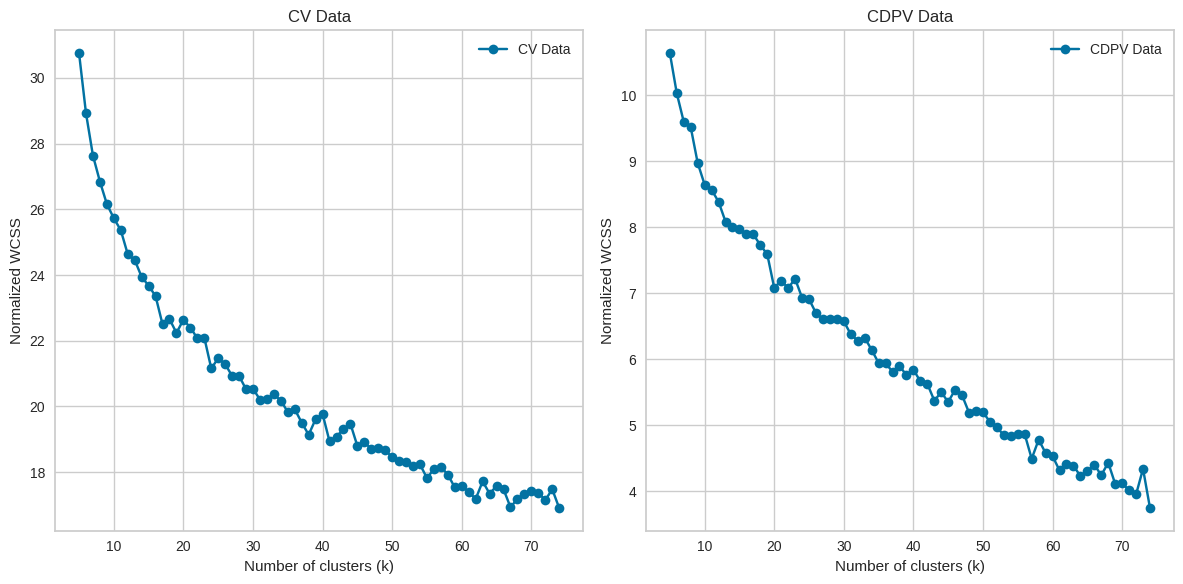
\includegraphics[width=1.0\textwidth]{figures/elbowmethod.png}
    \caption{K-Means Elbow Method}
    \label{elbow}
    Plots show no obvious choice for K
\end{figure}
The Silhouette method is used to analyze promising values to aid the decision-making process. A cluster with a value of one means points are perfectly assigned in a cluster, and clusters are easily distinguishable. Zero means clusters overlap; negative one means points are assigned to the wrong cluster. The K value should be chosen based on which value produces the most clusters with Silhouette scores greater than the average score of the dataset, represented by the red-dotted line seen in Figure \ref{cv_silhouette} and Figure \ref{dpv_silhouette}. Furthermore, there should not be wide fluctuations in the size of the clusters. The width of the clusters represents the number of data points belonging to the cluster. 
\begin{figure}[!h]
  	\centering
  	\begin{subfigure}{1.0\textwidth}
    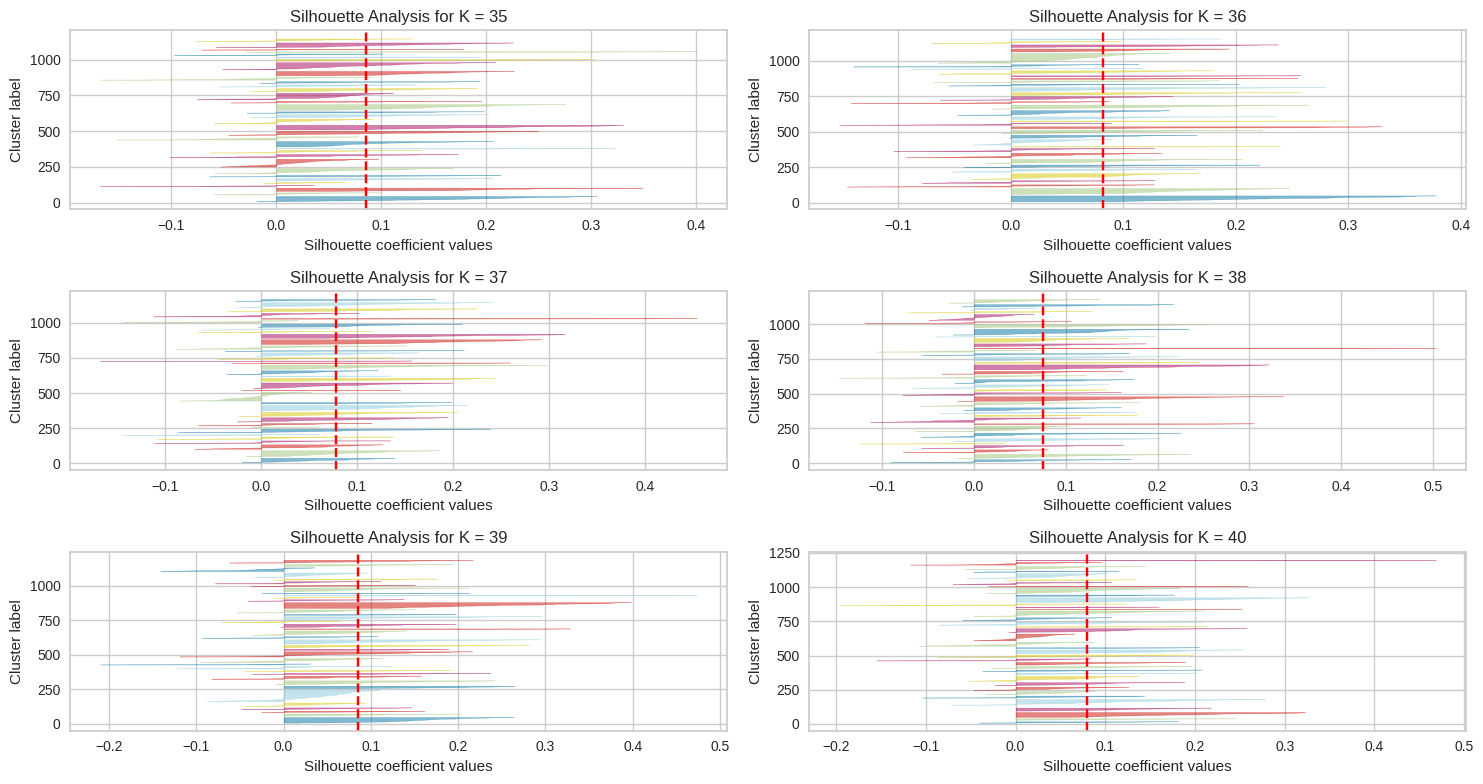
\includegraphics[width=1.0\textwidth]{figures/cv_silhouette.png}
    \caption{CV Silhouette Method}
    \label{cv_silhouette}
    \end{subfigure}
    
    \begin{subfigure}{1.0\textwidth}
    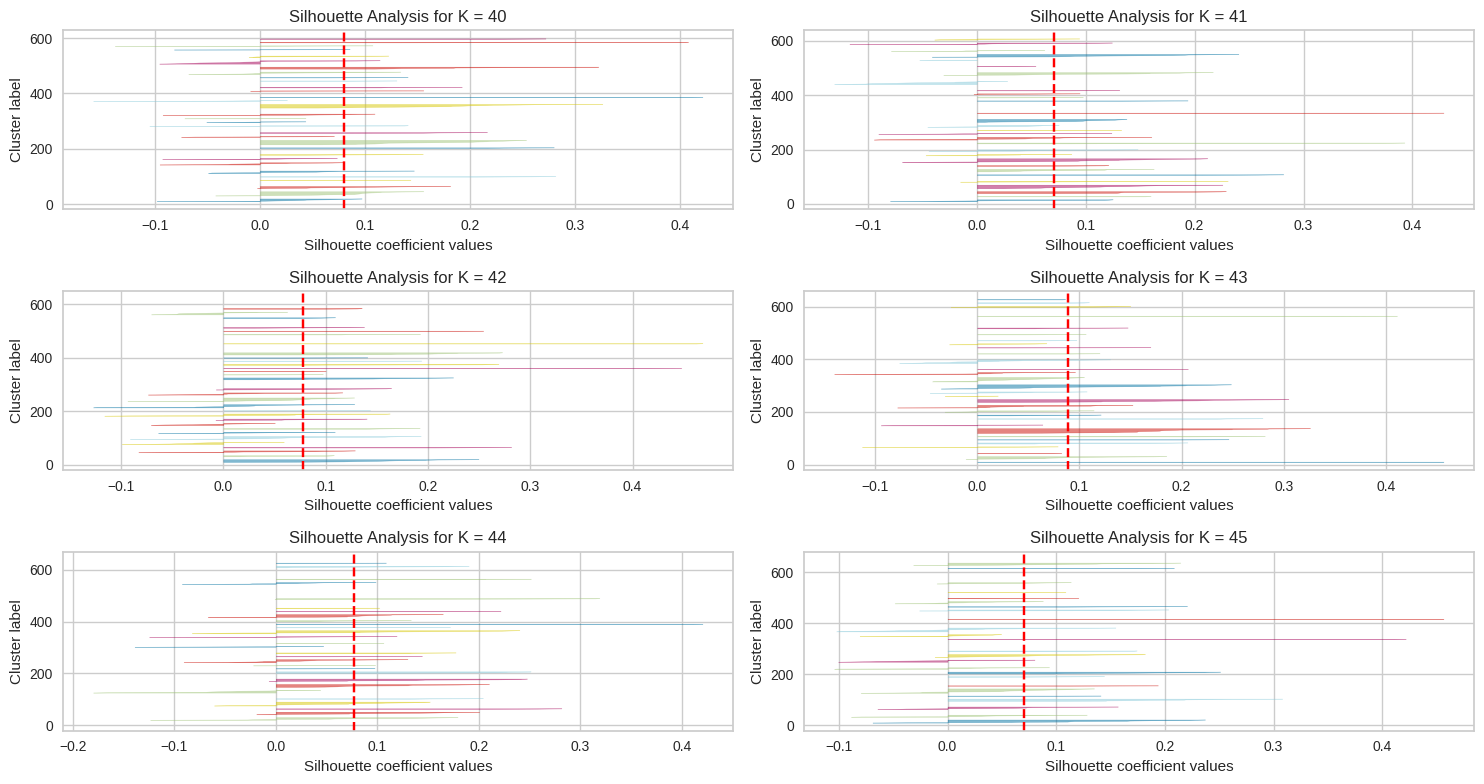
\includegraphics[width=1.0\textwidth]{figures/dpv_silhouette.png}
    \caption{DPV Silhouette Method}
    \label{dpv_silhouette}
    \end{subfigure}
    
    \caption{Silhouette Method for Promising K Values}
\end{figure}
In Figure \ref{cv_silhouette}, which showcases the application of the Silhouette method for CV cross-validation, K = 38 yields the highest number of clusters with a score surpassing the mean of the dataset. This configuration reduces the number of clusters scoring below zero and minimizes the variance in cluster sizes.
Similarly, in Figure \ref{dpv_silhouette} showcasing the Silhouette method for DPV, K = 42 results in the best quality of clusters. A subset of the cluster results is available in the appendix. Despite having 100 different combinations of metals and ligands, using a relatively small K value still shows promising results, as the data points within each cluster have similar overall shapes, which is crucial for compound identification. 

\begin{figure}[!h]
  \centering
  	\begin{subfigure}{1.0\textwidth}
  	\centering
    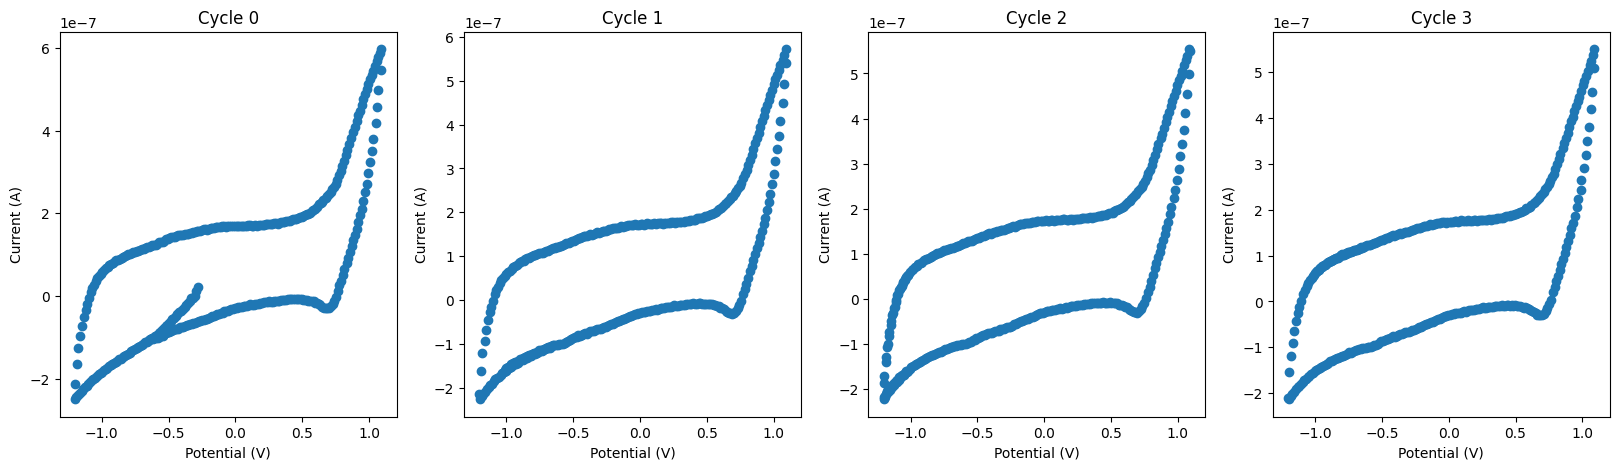
\includegraphics[width=0.8\textwidth]{figures/dbscan_results.png}
    \caption{Cluster 1}
    \end{subfigure}
    
    \begin{subfigure}{1.0\textwidth}
    \centering
    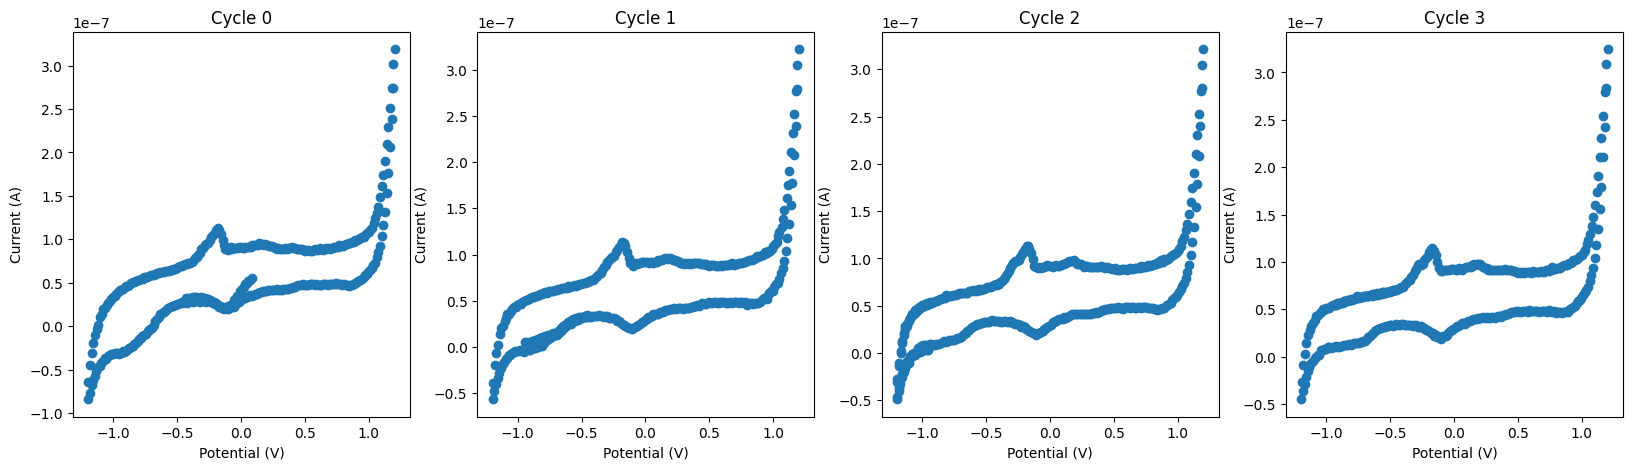
\includegraphics[width=0.8\textwidth]{figures/dbscan_results1.png}
    \caption{Cluster 2}
    \end{subfigure}
    
    \begin{subfigure}{1.0\textwidth}
    \centering
    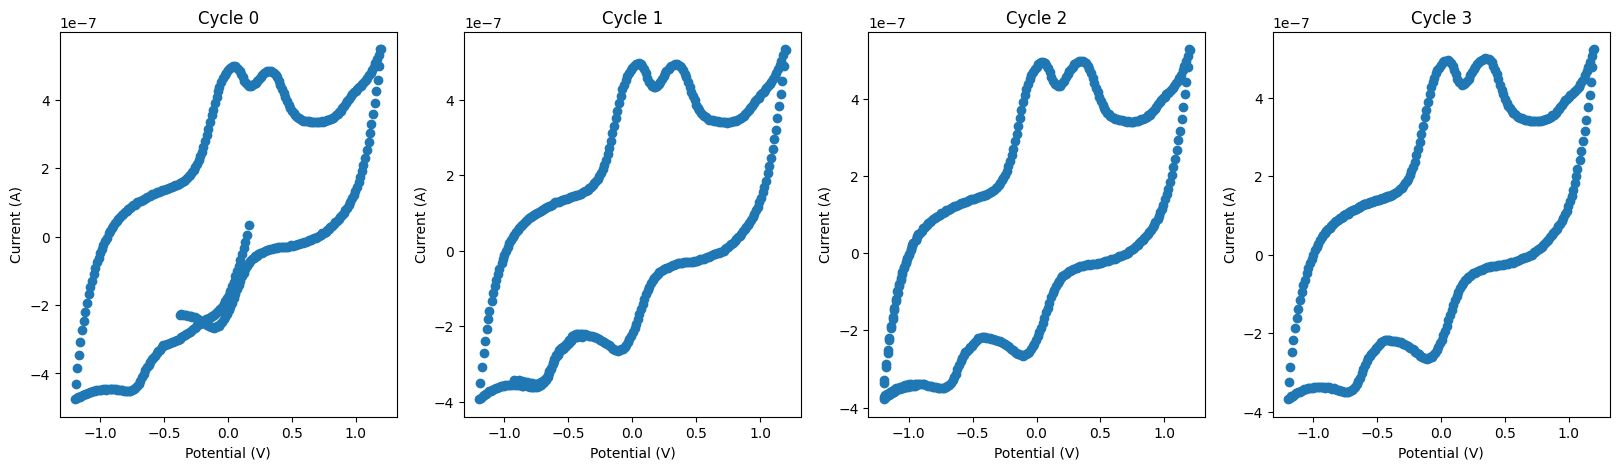
\includegraphics[width=0.8\textwidth]{figures/dbscan_results2.png}
    \caption{Cluster 3}
    \end{subfigure}
    
    \begin{subfigure}{1.0\textwidth}
    \centering
    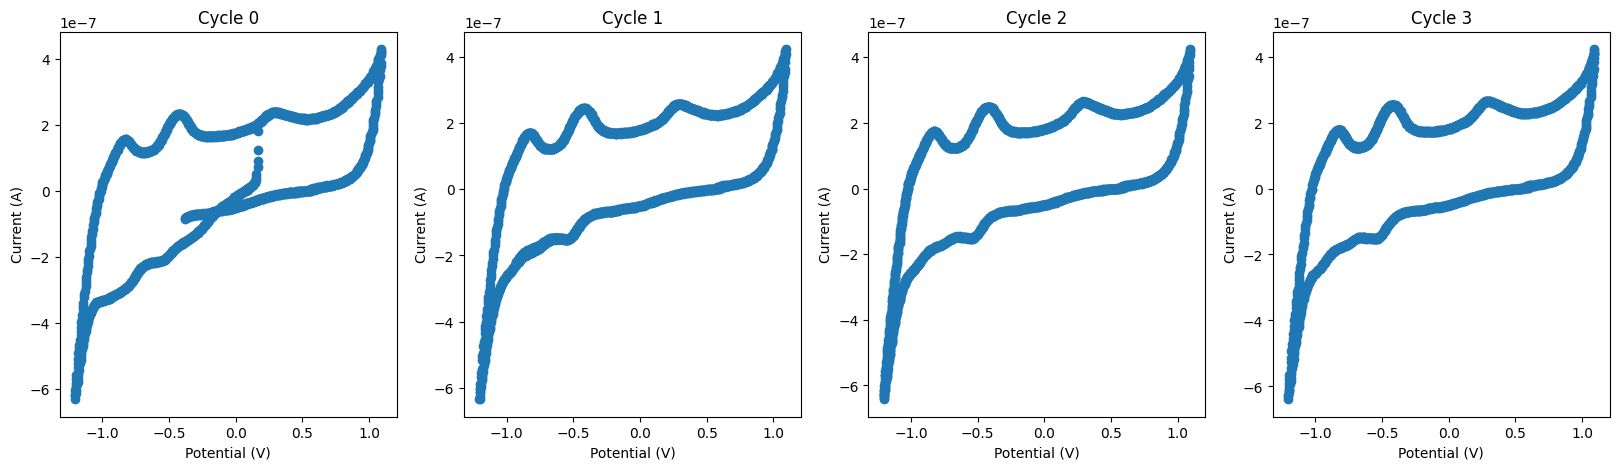
\includegraphics[width=0.8\textwidth]{figures/dbscan_results3.png}
    \caption{Cluster 4}
    \end{subfigure}
    
    \caption{DBSCAN Clusters}
    \label{dbscan_results}
\end{figure}
DBSCAN, as an alternative clustering method, demonstrated significant promise in identifying anomalous data points. With the appropriate parameters, DBSCAN efficiently grouped cycles from the same experiment. As Figure \ref{dbscan_results} depicts, DBSCAN defines a cluster comprising cycles solely from a single experiment. This capability could be seamlessly incorporated into SDLs as an error validation mechanism. Any cycle not assigned to the same cluster as others from the identical experiment could trigger an error notification, prompting intervention and investigation. Another method is identifying the erroneous clusters and investigating the assigned data points, as seen in Figure \ref{error_detection}.
\begin{figure}[!h]
  \centering
    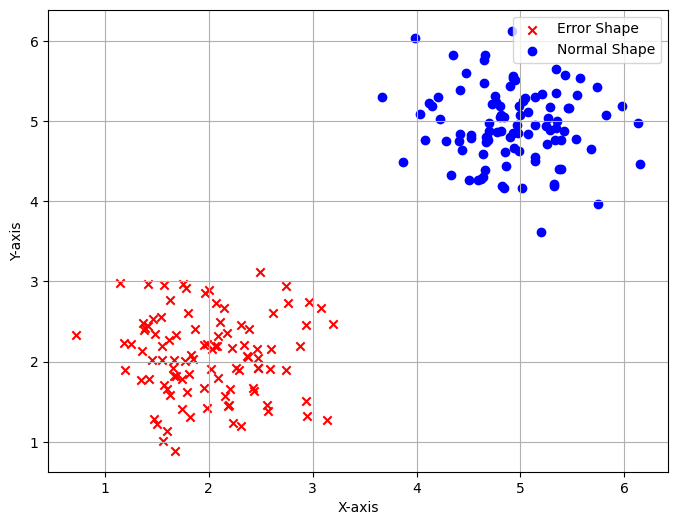
\includegraphics[width=0.8\textwidth]{figures/error_detection.png}
    \caption{UMAP Visualization of Normal CV Data and Incorrectly Shaped Data}
    \label{error_detection}
\end{figure}
To further demonstrate the efficacy of the encoding, t-SNE and UMAP projections are created to visualize the data in 2-D and show how the shapes, metals, and ligands are distributed. 
\begin{figure}[!h]
  \centering
    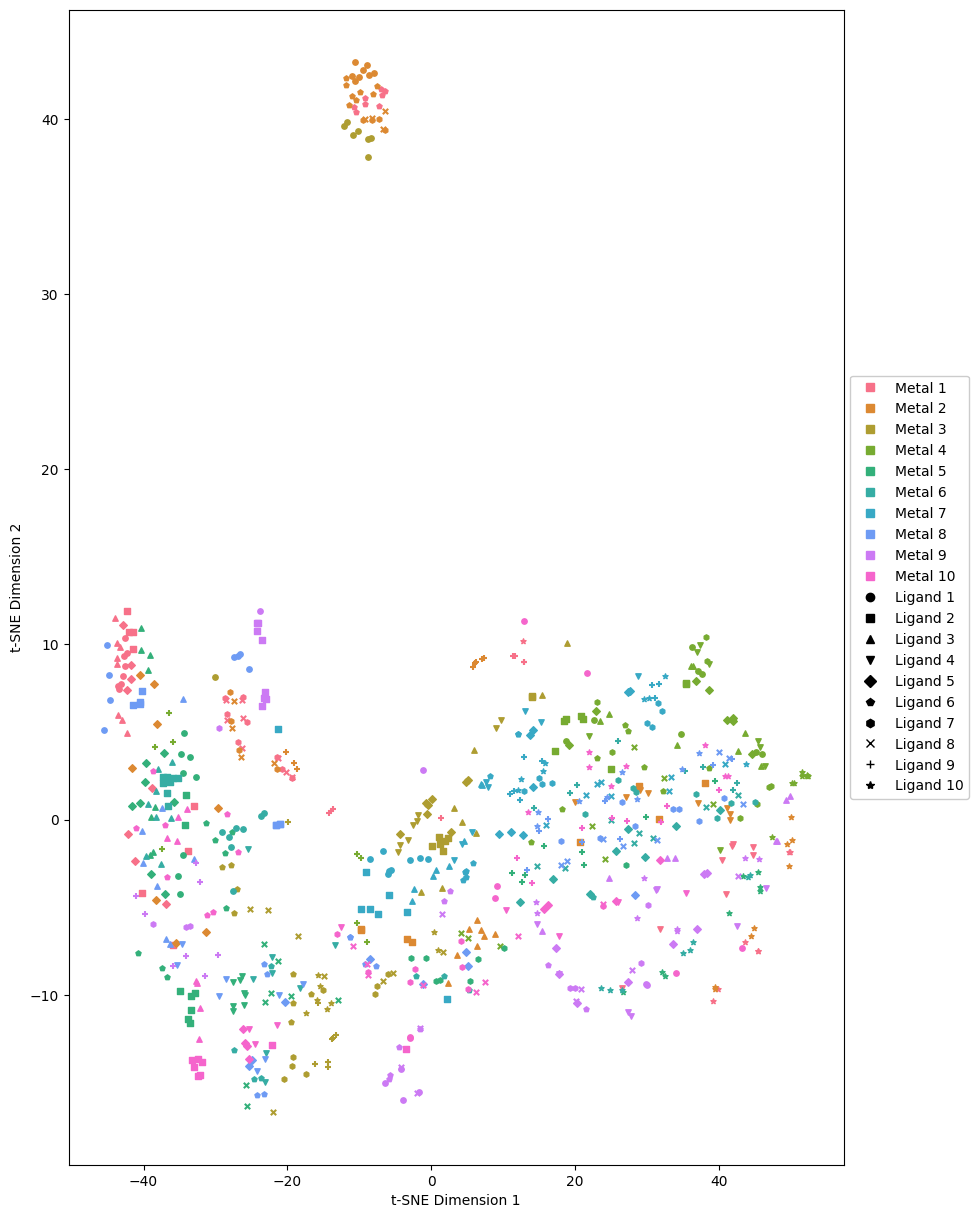
\includegraphics[width=1.0\textwidth]{figures/cv_tsne.png}
    \caption{Cyclic Voltammetry t-SNE Projection}
    \label{cv-tsne}
\end{figure}
\begin{figure}[!h]
  \centering
    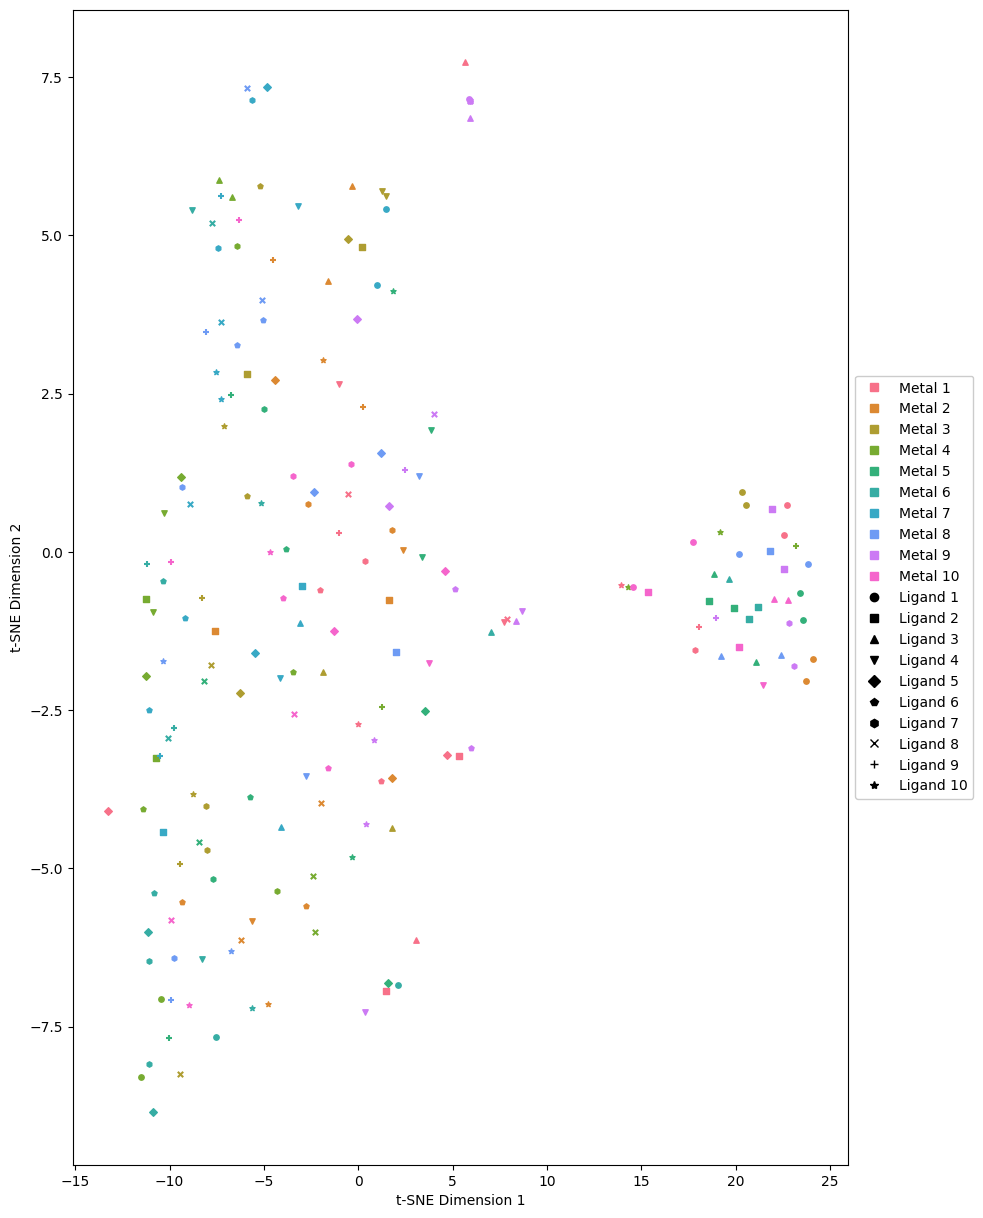
\includegraphics[width=1.0\textwidth]{figures/dpv_tsne.png}
    \caption{Differential Pulse Voltammetry t-SNE Projection}
    \label{dpv-tsne}
\end{figure}
As seen in Figure \ref{cv-tsne} and Figure \ref{dpv-tsne}, t-SNE emphasizes local structure and tends to agglomerate similar data points into tight clusters. As a result, t-SNE plots often show clearer separation between clusters but may not preserve the global structure as effectively. t-SNE primarily preserves local neighbourhoods, which leads to tighter clusters of similar points. However, it may not always capture the global structure accurately, especially for complex datasets. t-SNE embeddings can vary significantly with different random initializations and parameter choices, making it less stable and potentially more sensitive to noise in the data. 
\begin{figure}[H]
  \centering
    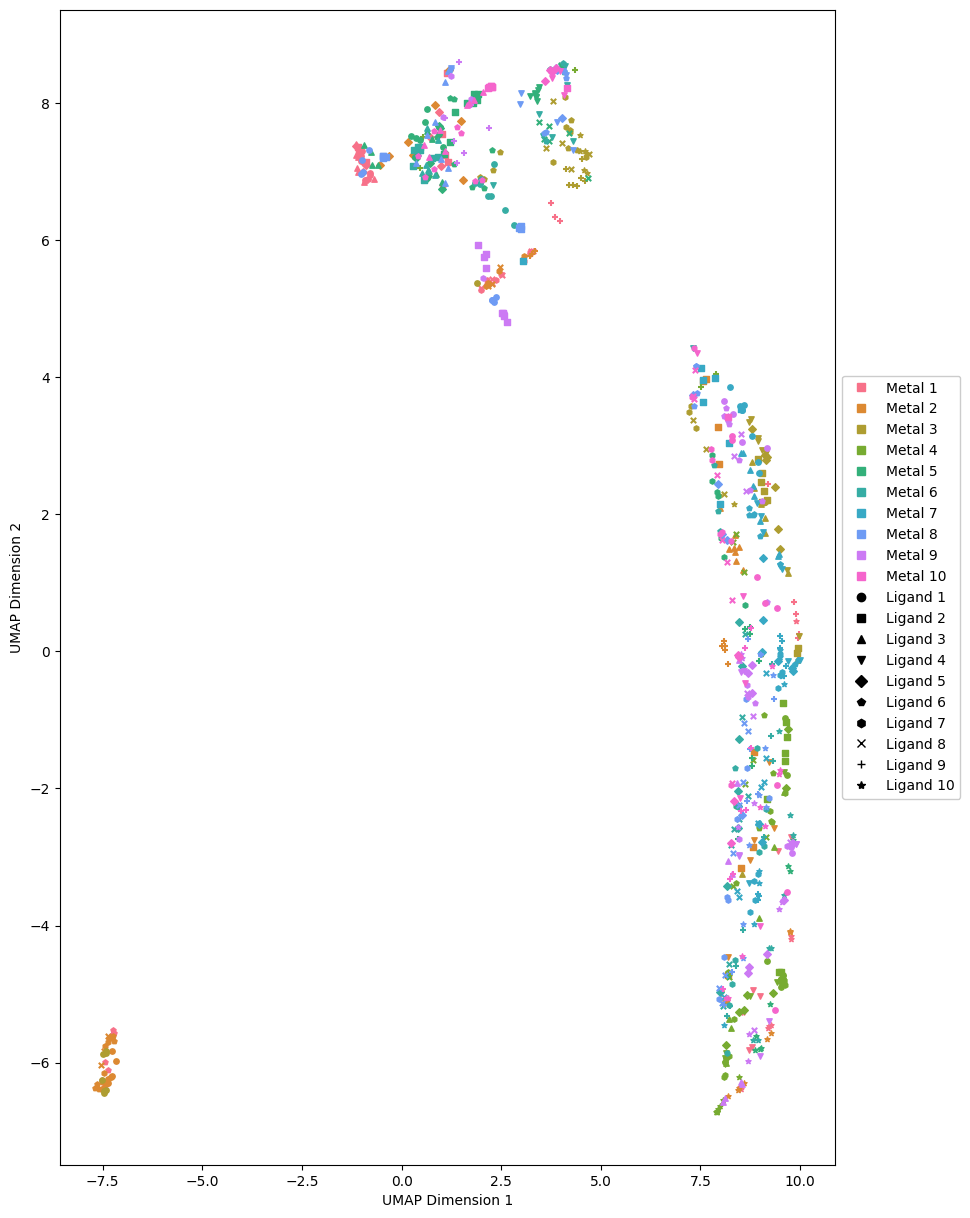
\includegraphics[width=1.0\textwidth]{figures/cv_umap.png}
    \caption{Cyclic Voltammetry UMAP Projection}
    \label{cv-umap}
\end{figure}
\begin{figure}[H]
  \centering
    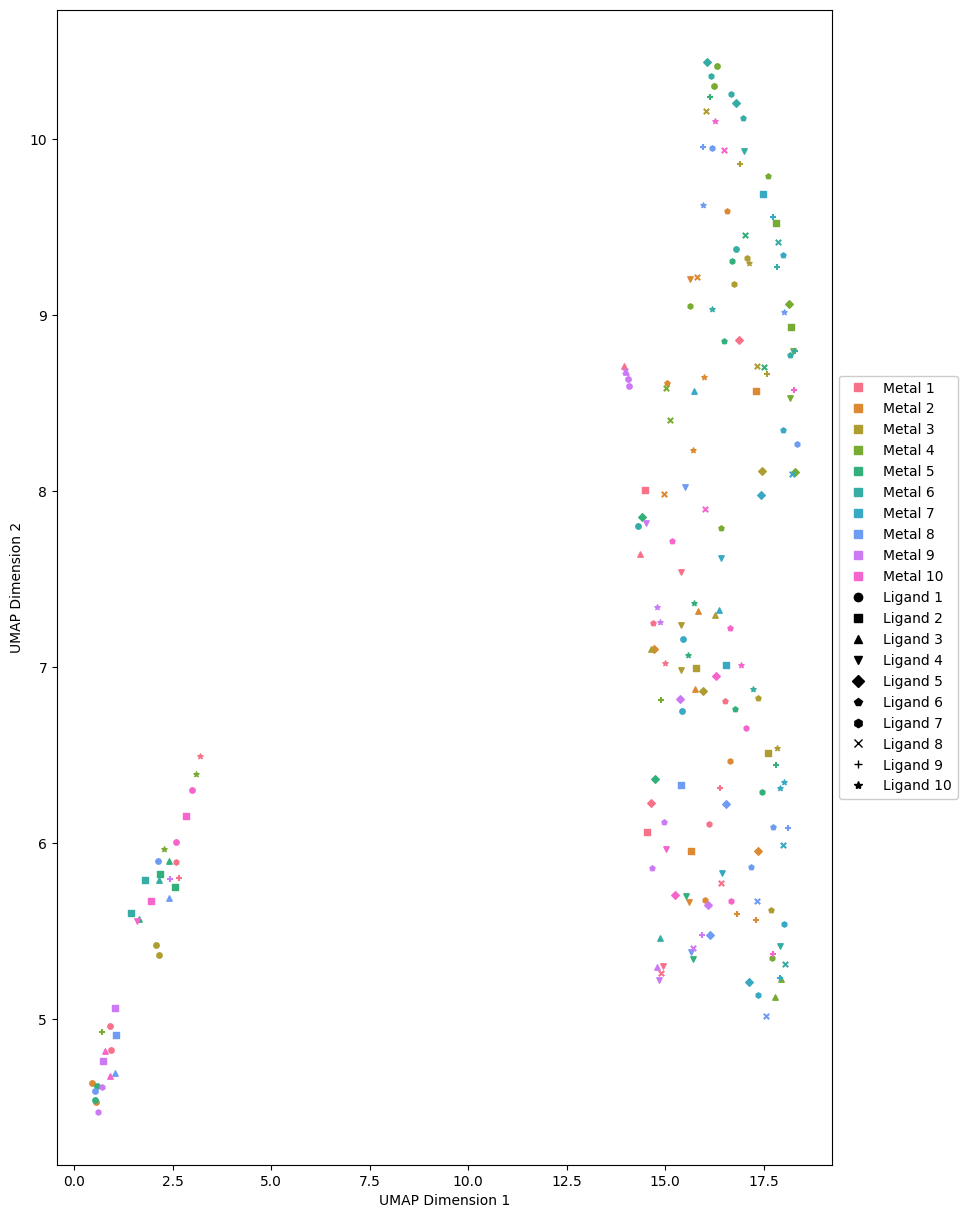
\includegraphics[width=1.0\textwidth]{figures/dpv_umap.png}
    \caption{Differential Pulse Voltammetry UMAP Projection}
    \label{dpv-umap}
\end{figure}
UMAP tends to focus more on preserving global structure and maintaining relative distance between clusters. Therefore, clusters in the UMAP plot are usually well-separated and evenly distributed. UMAP tries to preserve local and global neighbourhoods, resulting in more evenly spaced clusters and better representation of local and global structures. UMAP embeddings are generally more stable across different runs and parameter settings than t-SNE. Figures \ref{cv-umap} and \ref{dpv-umap} illustrate these characteristics, especially when contrasted with the projections generated by t-SNE. For example, Figure \ref{cv-umap} clearly shows more evenly spaced clusters than Figure \ref{cv-tsne}. Interactive plots, as seen in Figure \ref{bokeh}, made with Bokeh, are available on \href{https://github.com/raineyfu/Thesis}{Github}. The corresponding voltammetry plot is shown when hovering over a point with the mouse. Pan, zoom, and rotation tools are also available. These plots are extremely useful for chemists as SDLs can automatically generate them.
\begin{figure}[!h]
  \centering
    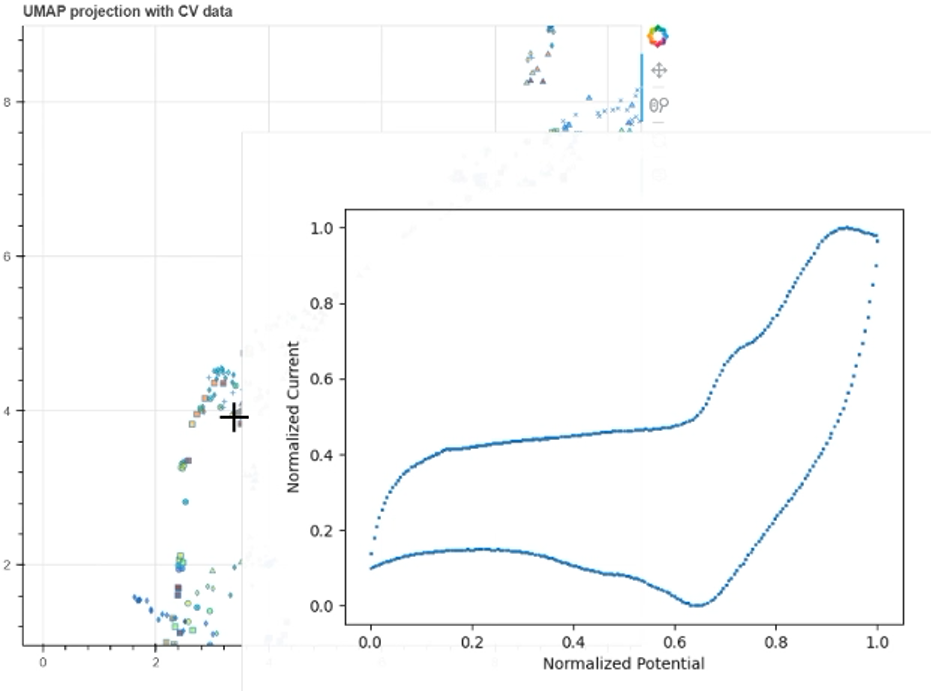
\includegraphics[width=1.0\textwidth]{figures/bokeh.png}
    \caption{Bokeh Interactive Plot with CV Data}
    \label{bokeh}
\end{figure}
Utilizing machine learning techniques to classify voltammetry data based on the overall shape presents numerous benefits over merely employing a script to identify the number of peaks, as has traditionally been done. Machine learning models can be trained to recognize patterns and variations regarding the overall shape and number of peaks. They can adapt to experimental conditions, electrode materials, and analytes without needing manual adjustment of parameters. Voltammetry data can often be noisy, especially at low concentrations. ML models can be trained to distinguish true peaks from noise more effectively than simple peak-finding algorithms. Voltammograms can vary in characteristics due to electrode deterioration, surface roughness, and solution composition. ML models can learn to handle this variability and provide more reliable peak classification across different experimental conditions. Additionally, ML models can learn when the electrode deteriorates and automatically polish it. ML models can automatically extract relevant features from voltammogram data, such as peak heights, peak widths, peak potential, and overall shape. This allows for more comprehensive analysis beyond locating peaks. Once trained, ML models can be integrated into larger data analysis pipelines to classify cyclic voltammetry data rapidly and efficiently, potentially saving time and effort compared to manual analysis or parameter tuning for peak-finding algorithms. These automated analysis techniques can be integrated into an SDL, updating them with newly generated data to increase accuracy as more experiments are performed.

In summary, clustering techniques are crucial in analyzing and interpreting experimental voltammetry results obtained from SDLs. By organizing data into meaningful clusters, clustering techniques like K-Means and DBSCAN and dimensionality reduction techniques like t-SNE and UMAP uncover patterns, similarities, and trends that enhance our understanding of the electrochemical compounds of interest. Choosing appropriate clustering algorithms and parameter selection methods, such as the Elbow and Silhouette Method, have been discussed to ensure meaningful and reliable clustering results. The results obtained from clustering algorithms and dimensionality reduction techniques have provided valuable insights into the underlying structure of the experimental data, facilitating compound identification, error detection, and decision-making processes in SDLs.